%% -*- coding: utf-8 -*-
\documentclass[12pt,a4paper]{report}
\usepackage[left=2cm,right=2cm,
    top=2cm,bottom=2cm,bindingoffset=0cm]{geometry} 
\usepackage[utf8]{inputenc}
\usepackage[english,russian]{babel}
\usepackage{indentfirst}
\usepackage{misccorr}
\usepackage{graphicx}
\usepackage{amsmath}
\usepackage{amsfonts}
\usepackage{amssymb}
\setcounter{page}{2}
\begin{document}

\begin{titlepage}
\newpage
  \begin{center}
     
    Санкт-Петербургский Политехнический Университет Петра Великого \\
    
    Институт компьютерных наук и технологий \\
    
    Кафедра компьютерных систем и программных технологий
    \end{center}
    
    \vspace{15em}
    \begin{center}
    \textsc{Лабораторная работа №4, №5}\\
    \vspace{5mm}
    \textsc{Аналоговая, частотная и фазовая модуляция}
    	
   \end{center}
\vspace{10em}

\newlength{\ML}
\settowidth{\ML}{«\underline{\hspace{0.7cm}}» \underline{\hspace{2cm}}}
\hfill\begin{minipage}{0.45\textwidth}
\vfill
  Руководитель \\
  \\
  \underline{\hspace{\ML}} Богач Н.\,В.\\
 
\end{minipage}%
\bigskip

\hfill\begin{minipage}{0.45\textwidth}
  Выполнил\\
  \\
  \underline{\hspace{\ML}} Солдатова Е.\,И.\\
  группа 33501/3
\end{minipage}%

\vspace{\fill}
\begin{center}
    
  Санкт-Петербург\\
   2018 
\end{center}
\end{titlepage}

\paragraph{1. Цель работы\\\\}
Изучение амплитудной модуляции/демодуляции сигнала.

\paragraph{2. Постановка задачи\\}
\begin{enumerate}
\item Сгенерировать однотональный сигнал низкой частоты 
\item Выполнить амплитудную модуляцию (АМ) по закону \textit{u(t)=(1+MU\tiny{m}\normalsize{cos(\begin{math}\Omega\end{math}t))cos(\begin{math}\omega\end{math}\tiny{0}\normalsize{t}+\begin{math}\phi\end{math}\tiny{0}\normalsize)}} для различных значений глубины модуляции M. Используйте встроенную функцию
MatLab ammod.
\item Получить спектр модулированного сигнала.
\item Выполнить модуляцию с подавлением несущей 
\textit{u(t)=(1+MU\tiny{m}\normalsize{cos(\begin{math}\Omega\end{math}t))cos(\begin{math}\omega\end{math}\tiny{0}\normalsize{t}+\begin{math}\phi\end{math}\tiny{0}\normalsize)}}. Получить спектр.
\item Выполнить однополосную модуляцию:

\begin{figure}[h!]
\center{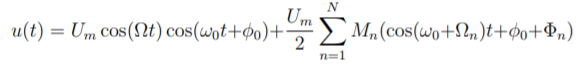
\includegraphics[width=0.7\linewidth]{1}}
\end{figure}

положив n=1

\item Выполнить синхронное детектирование и получить исходный однополосный сигнал.
\item Рассчитать КПД модуляции.

\begin{figure}[h!]
\center{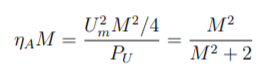
\includegraphics[width=0.3\linewidth]{2}}
\end{figure}

\item Выполнить фазовую модуляцию/демодуляцию по закону $u(t)=(U_{m}cos({\Omega}t+ks(t)) $, используя встроенную функцию Matlab pmmod, pmdemod

\item Выполнить частотную модуляцию/демодуляцию по закону
	
\begin{figure}[h]
\center{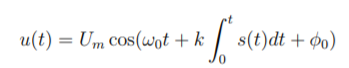
\includegraphics[width=0.45\linewidth]{3}}
\end{figure}
используя встроенные функции Matlab fmmod, fmdemod

\end{enumerate}

\paragraph{3. Теоретическая часть \\\\}

Модуляцией называют процесс преобразования одной либо нескольких характеристик модулирующего высокочастотного колебания при воздействии управляющего низкочастотного сигнала. В итоге спектр управляющего сигнала перемещается в высокочастотную область, где передача высоких частот является более эффективной.

Модуляция выполняется с целью передачи информации посредством электромагнитного излучения. Передаваемые данные содержатся в управляющем сигнале. А функцию переносчика осуществляет высокочастотное колебание, именуемое несущим. В роли несущего колебания могут быть использованы колебания разнообразной формы: пилообразные, прямоугольные и др., но обычно используют гармонические синусоидальные. Исходя из того, какая именно характеристика синусоидального колебания изменяется, различают несколько типов модуляции.

\textbf{Амплитудная модуляция\\}
На вход модулирующего устройства передают модулирующий и опорный сигналы, в результате на выходе имеем смодулированный сигнал. Условием корректного преобразования считается удвоенное значение несущей частоты в сравнении с максимальным значением полосы модулирующего сигнала. Данный тип модуляции достаточно прост в исполнении, но отличается невысокой помехоустойчивостью.

Коэффициент полезного действия данной модуляции равен отношению мощности боковых частот к общей средней мощности модулированного сигнала:

\begin{figure}[h!]
\center{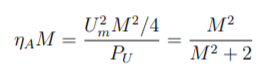
\includegraphics[width=0.3\linewidth]{2}}
\end{figure}

Как видно, основная доля мощности АМ – сигнала приходится на несущую частоту. При балансной модуляции (с подавлением несущей) производится перемножение двух сигналов – модулирующего и несущего, при котором происходит подавление несущего колебания, соответственно, КПД модуляции становится равным 100\%.

\textbf{Частотная модуляция\\}
В результате данного типа модуляции сигнал модулирует частоту опорного сигнала, а не мощность. Поэтому если величина сигнала увеличивается, то, соответственно, растет частота. Ввиду того, что полоса получаемого сигнала намного шире исходной величины сигнала.

\textbf{Фазовая модуляция\\}
В процессе данного типа модуляции модулирующий сигнал использует фазу опорного сигнала. При данном типе модулирования получаемый сигнал имеет достаточно широкий спектр, потому что фаза оборачивается на 180 градусов.\\

Демодуляцией называют процесс восстановления величин, вызвавших изменение параметров носителей при модуляции. Выполняется на принимающей стороне при известных условиях модуляции на передающей стороне.

\paragraph{4. Ход работы \\\\}
Зададим исходный сигнал. Затем по ходу работу проведем различные типы модуляции средствами MatLab.

Текст программы:\\\\
N=256;\\
t=0:0.01:2*pi;\\
f0=0.5;\\
fc=5;\\
fs=110;\\
x=awgn(cos(2*pi*f0*t),20);\\
figure;\\
plot(t,x);\\\\
\% Амплитудная модуляция\\
y=ammod(x, fc, fs, 0, 0.7);\\
figure;\\
subplot(2,1,1);\\
plot (x, y);\\
subplot(2,1,2);\\
plot(abs(fft(y, N)));\\\\
\% Амплитудная модуляция с подавлением несущей\\
y1=ammod(x, fc, fs);\\
figure;\\
subplot(2,1,1);\\
plot (x, y1);\\
subplot(2,1,2);\\
plot(abs(fft(y1, N)));\\\\
\%Однополосная модуляция
z=ssbmod(x,fc,fs,0,'upper');\\
figure;\\
subplot(4,1,1);\\
plot (t, x);\\
subplot(4,1,2);\\
plot (t, z);\\
subplot(4,1,3);\\
plot(abs(fft(z, N)));\\
xorig = demod(z,fc,fs);\\
subplot(4,1,4);\\
plot(t,xorig);\\\\
\%КПД модуляции
M = fc/0.7;\\
kpd = M\^2/(M\^2 + 2)\\\\
\%Фазовая модуляция\\
y\_pm=pmmod(x,fc,fs,pi/2);\\
figure;\\
subplot(3,1,1);\\
plot(t,x,'r',t,y\_pm,'m');\\
subplot(3,1,2);\\
plot(abs(fft(y\_pm, N)));\\
\%Фазовая демодуляция\\
y\_pmd=pmdemod(y\_pm,fc,fs, pi/2);\\
subplot(3,1,3);\\
plot(t,x,'.-',t,y\_pmd,'m');\\\\
figure;\\
y\_fm=fmmod(x,fc,fs,3);\\
subplot(3,1,1);\\
plot(t,x,'r',t,y\_fm,'m');\\
subplot(3,1,2);\\
plot(abs(fft(y\_fm, N)));\\
y\_fmd=fmdemod(y\_fm,fc,fs, 3);\\
subplot(3,1,3);\\
plot(t,x,'.-',t,y\_fmd,'m');\\


Исходный сигнал:

\begin{figure}[h]
\center{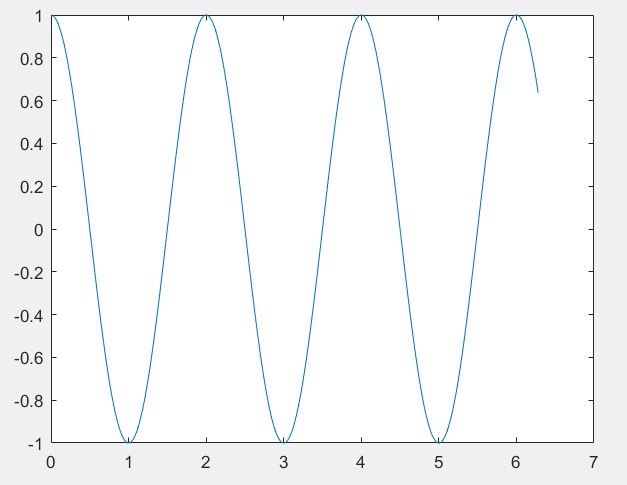
\includegraphics[width=0.5\linewidth]{sig}}
\end{figure}

Результаты амплитудной модуляции и спектр модулированного сигнала:

\begin{figure}[h]
\center{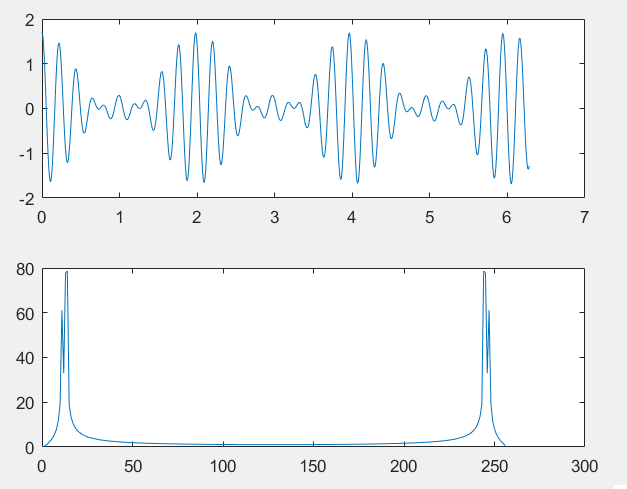
\includegraphics[width=0.5\linewidth]{ammod}}
\end{figure}
\newpage
Результаты амплитудной модуляции c подавлением несущей и спектр модулированного сигнала:

\begin{figure}[h!]
\center{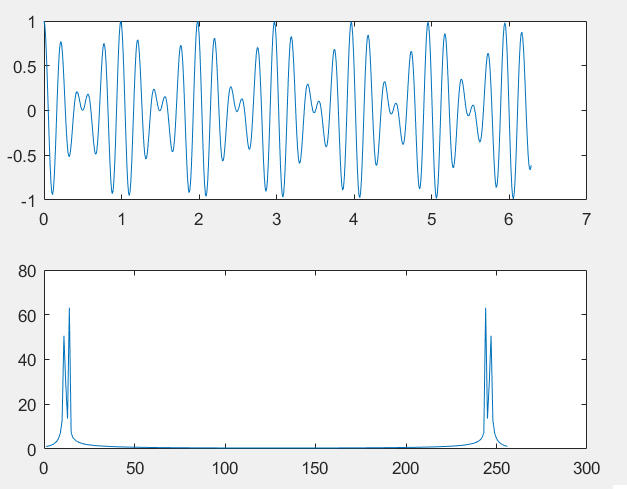
\includegraphics[width=0.5\linewidth]{ammod1}}
\end{figure}

Результаты однополосной модуляции с последующим синхронным детектированием и получением исходного однополосного сигнала:

\begin{figure}[h]
\center{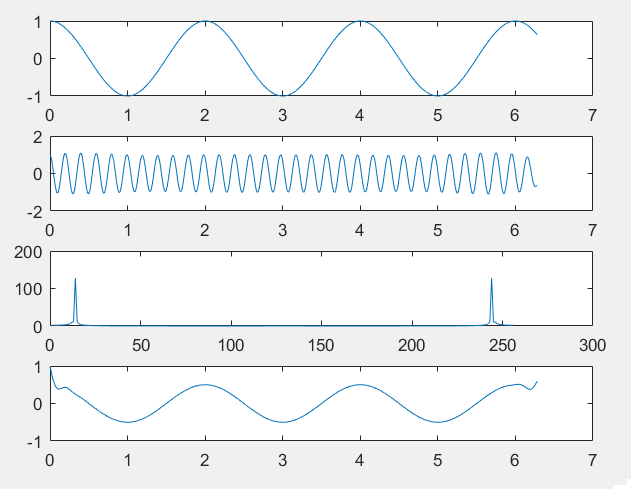
\includegraphics[width=0.5\linewidth]{ssbmod}}
\end{figure}

Получили КПД модуляции равным 96,23\%.
\newpage
Результаты фазовой модуляции при помощи встроенной функции pmmod, спектр модулированного сигнала и результаты демодуляции:

\begin{figure}[h!]
\center{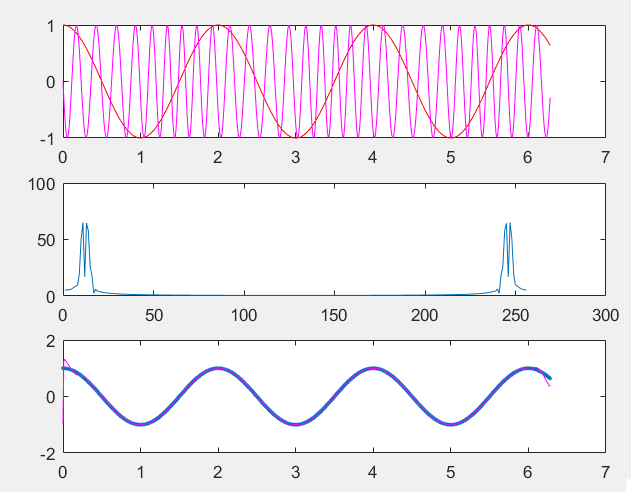
\includegraphics[width=0.5\linewidth]{pmmod}}
\end{figure}

Результаты модуляции при помощи встроенной функции fmmod, спектр модулированного сигнала и результаты демодуляции:

\begin{figure}[h!]
\center{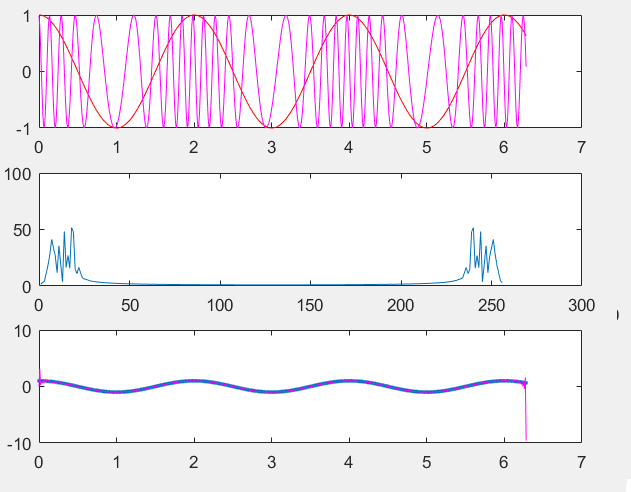
\includegraphics[width=0.5\linewidth]{fmmod}}
\end{figure}

\paragraph{5. Выводы \\\\}
Амплитудная модуляция применяется в системах телевизионного вещания,
в системах звукового радиовещания и радиосвязи на длинных и средних волнах, в системе трехпрограммного проводного вещания.

Особенностью модулированного сигнала является наличие в спектре двух боковых полос несущих одинаковую информацию. Подавление одной из полос позволяет уменьшить спектр модулированного сигнала и, соответственно, увеличить число каналов в линии связи. Модуляция при которой формируется модулированный сигнал с одной боковой полосой (верхней или нижней) называется однополосной. 

Частотная модуляция применяется для высококачественной передачи звукового (низкочастотного) сигнала в радиовещании (в диапазоне УКВ), для звукового сопровождения телевизионных программ, передачи сигналов цветности в телевизионном стандарте SECAM, видеозаписи на магнитную ленту, музыкальных синтезаторах.

Фазовая модуляция не нашла применения в радиотехнических системах, но в фотоэлектрических системах используется широко.

Сравнивая спектры всех модулированных сигналов можно отметить, что наибольшую ширину имеет спектр ЧМн сигнала, наименьшую — АМн, ФМн.

\end{document}